\documentclass[9pt,twoside]{pnas-new}
\usepackage{hyperref}

\articletype{Research Article}

\templatetype{pnasmathematics}

\begin{document}

\title{Do Constitutions Shape Democracy? A Machine Learning Analysis of Constitutional Design and Democratic Performance}

\author[a,1]{Rishith Hakker}

\affil[a]{Department of Quantitative Social Science, Dartmouth College, Hanover, NH 03755}

\leadauthor{Hakker}

\significancestatement{After Egypt's 2011 uprising, reformers wrote executive constraints and judicial independence into the new constitution. After Lebanon's civil war, the Taif Agreement encoded confessional power-sharing. Neither produced durable democracy. This paper provides systematic evidence for why: when a machine learning model is trained on nearly 17,000 country-year observations, the constitutional provisions that best predict democracy are not separation of powers or judicial independence---the classical Madisonian safeguards---but political competition, institutional accountability, and civil liberties. These findings illuminate a fundamental de facto versus de jure divide: writing the right provisions into constitutional text is insufficient when the political conditions that make those provisions enforceable are absent. The gap between what a country's constitution promises and what it actually delivers is a measurable diagnostic indicator of the distance between constitutional design and democratic reality---widest in newly adopted constitutions and in regimes where norms and enforcement capacity have not consolidated.}

\authorcontributions{R.H.\ designed the study, constructed the constitutional typology, built and trained all models, and wrote the paper.}
\authordeclaration{The author declares no competing interests. Code, data, and replication materials are available at \href{https://github.com/rishithakker27/constitution-democracy}{github.com/rishithakker27/constitution-democracy} (AI chat transcripts are in GitHub). Project website: \href{https://portfolio-eight-lilac-55.vercel.app}{portfolio-eight-lilac-55.vercel.app}.}
\correspondingauthor{\textsuperscript{1}Correspondence: rishith.hakker@dartmouth.edu}

\keywords{Constitutional design $|$ Democratic backsliding $|$ Machine learning $|$ De facto constitutionalism $|$ V-Dem}

\begin{abstract}
What does constitutional text actually tell us about democracy? We address this question using a machine learning framework applied to 17,390 country-year observations spanning 1789--2023. We score each country-constitution dyad on 14 structural dimensions using an LLM-assisted typology applied to the Comparative Constitutions Project (CCPCNC v5), then train a gradient-boosted model (CatBoost) with country-blocked five-fold cross-validation to predict V-Dem Polyarchy scores from constitutional features alone. Constitutional text contains real but limited predictive information: the model achieves a fold-average $R^2$ of $0.10 \pm 0.09$ and mean absolute error of $0.22$ on the 0--1 Polyarchy scale on entirely held-out countries. The most striking finding is in the feature rankings: Political Competition (10.7\%), Institutional Accountability (9.2\%), and Civil Liberties (8.7\%) are the top predictors, while the classical Madisonian safeguards---Executive Constraints (6.8\%), Judicial Independence (5.1\%), and Legislative Autonomy (4.5\%)---rank in the bottom half. We further construct a \emph{constitutional gap}---the difference between constitutionally predicted and actually achieved democracy---and show that this gap is largest in newer constitutions and in regimes where democratic norms and enforcement capacity have not yet consolidated, while countries with older constitutional orders consistently outperform their text. Much of the variation unexplained by constitutional text appears to be structured by extra-textual institutional and cultural conditions rather than being random noise.
\end{abstract}

\dates{This manuscript was compiled on \today}

\maketitle
\thispagestyle{firststyle}
\ifthenelse{\boolean{shortarticle}}{\ifthenelse{\boolean{singlecolumn}}{\abscontentformatted}{\abscontent}}{}

\Firstpage

James Madison believed that the structural architecture of government---separated powers, bicameralism, an independent judiciary---would be the primary safeguard of democratic liberty. Two centuries later, constitution-writers from Cairo to Beirut have followed this blueprint, encoding judicial independence, executive constraints, and legislative autonomy into documents adopted in the wake of authoritarian rule or civil conflict. Yet democracy has not reliably followed. This paper asks, empirically and at scale, which constitutional provisions actually predict democratic outcomes---and the answer departs markedly from the Madisonian template.

\Endparasplit

\section*{Introduction}

The central question in constitutional design is whether text matters. Constitutionalists in the Madisonian tradition argue that structural provisions---separation of powers, judicial independence, executive constraints---constrain elite behavior and protect democratic governance by making it costly to concentrate authority. Critics counter that constitutions are endogenous documents: they reflect the political settlements that powerful actors were willing to accept at the time of drafting, and provisions that conflict with those actors' interests are simply circumvented or ignored. On this view, the causal arrow runs from underlying political conditions to constitutional text, not the other way around.

Both positions find support in comparative case evidence. What has been missing is a systematic, large-$n$ empirical test of which constitutional provisions carry predictive information about democratic outcomes---one that does not rely on researcher selection of variables, can handle the complexity of hundreds of constitutional provisions simultaneously, and evaluates predictions out-of-sample on entirely unseen countries. We provide that test.

Our approach rests on a three-stage pipeline. First, we map the raw variables of the Comparative Constitutions Project onto 14 theoretically motivated constitutional dimensions using an LLM-assisted typology. Second, we score each of 17,390 country-years on all 14 dimensions. Third, we train a gradient-boosted model with country-blocked cross-validation to predict V-Dem Polyarchy scores from these dimensional scores, generating out-of-fold predictions that serve as each country's ``constitutionally implied'' democracy level.

The results produce two interrelated findings that together make a strong case for the de facto versus de jure distinction in constitutional politics. First, when the model is allowed to weight features freely, the classical Madisonian provisions---executive constraints, judicial independence, legislative autonomy---rank near the \emph{bottom} of the feature importance distribution. The top-ranked features are Political Competition (10.7\%), Institutional Accountability (9.2\%), and Civil Liberties (8.7\%). Provisions governing the real structure of political competition are far more predictive of democratic outcomes than provisions governing the formal architecture of government.

Second, the constitutional gap---the signed difference between constitutional promise and democratic reality---is not random noise. Newer constitutions are systematically associated with larger gaps than older ones. The democratic culture that makes constitutional provisions enforceable takes decades to develop; text alone cannot substitute for it.

Together, these findings cast doubt on constitutional engineering as a reliable path to democracy. When Egypt's post-2011 constitution encoded judicial independence and executive constraints, or when Lebanon's elite negotiations under the Taif Agreement tried to redistribute power through constitutional text, the missing ingredient was not the right provisions---it was the de facto political competition and accountability that would have made those provisions meaningful.

The safest summary of the paper's contribution is this: \textit{constitutional text contains modest but real predictive information about democratic performance, but much of the variation appears to be structured by extra-textual institutional and cultural conditions that provisions alone cannot supply.}

The remainder of the paper proceeds as follows. Section~2 develops the theoretical framework and formal hypotheses. Section~3 describes the data, LLM-assisted typology, and robustness validation. Section~4 presents the Polyarchy prediction results. Section~5 examines which provisions matter most and compares predictability across V-Dem's five democracy concepts. Section~6 constructs the constitutional gap, presents illustrative cases, and examines constitutional age. Section~7 tests whether democratic culture explains additional variance. Section~8 discusses findings and limitations. Section~9 concludes.

% ---------------------------------------------------------------
\section*{Literature Review}

The debate over whether constitutional design shapes democratic outcomes has two deeply entrenched camps. The Madisonian tradition, rooted in Federalist No.~51, holds that structural provisions---separated powers, an independent judiciary, bicameralism---constrain the ambitions of would-be autocrats by making it costly to concentrate authority. This view has informed a large comparative literature linking specific constitutional choices to institutional performance. Persson and Tabellini \cite{persson_tabellini_2003} find that presidential systems and majoritarian electoral rules are associated with smaller governments and different fiscal outcomes, while North and Weingast \cite{north_weingast_1989} argue that credible constitutional commitments enabled the financial revolution in seventeenth-century England by making property rights enforceable against the Crown. The underlying logic is that text, if properly designed, alters incentives by making deviations costly and observable.

The skeptical tradition disputes the direction of causality. On this view, constitutions are endogenous documents: they reflect the balance of power among elites at the moment of drafting and encode the compromises those elites were willing to accept. Provisions that powerful actors do not want enforced are simply not enforced. Ginsburg and Simpser \cite{ginsburg_simpser_2014} document that many authoritarian constitutions contain elaborate democratic provisions, serving primarily as window-dressing for international audiences rather than meaningful constraints on behavior. The most influential formalization of this argument is Acemoglu and Robinson's \cite{acemoglu_robinson_2006} distinction between de jure and de facto political power: even when formal institutions change, outcomes track the underlying distribution of de facto power, which constitutional text cannot alter on its own. This paper's empirical design is a direct test of that distinction at scale.

The comparative constitutions literature provides the data infrastructure that makes such tests possible. Elkins, Ginsburg, and Melton \cite{elkins_ginsburg_melton_2009} assembled the Comparative Constitutions Project, tracking the content and survival of every national constitution since 1789 and documenting systematic patterns in constitutional design, diffusion, and endurance. Their finding that constitutional longevity correlates with democratic stability anticipates the age effects we document here. On the measurement of democratic outcomes, we rely on the V-Dem project \cite{coppedge_vdem_2024}, which offers fine-grained, expert-coded indices across five democracy concepts---far richer than binary regime classifications and better suited to detecting the gradations that distinguish electoral from liberal from egalitarian democracy.

The democratic backsliding literature provides the applied motivation. Levitsky and Ziblatt \cite{levitsky_ziblatt_2018} and Bermeo \cite{bermeo_2016} document how contemporary democratic erosion typically proceeds through the gradual hollowing out of institutions by elected leaders rather than outright coups---a process in which constitutional text is nominally intact while de facto democratic performance deteriorates. This pattern is precisely what the constitutional gap captures. Finally, our methodological approach draws on the growing use of machine learning in political science: Grimmer, Roberts, and Stewart \cite{grimmer_roberts_stewart_2022} provide a framework for deploying text and predictive models in social science settings with appropriate out-of-sample discipline, which informs our use of country-blocked cross-validation throughout.

\section*{Methodology}

\subsection*{Data}

We draw on two primary datasets. The \textbf{Comparative Constitutions Project CCPCNC v5} \cite{elkins_ginsburg_melton_ccpc} provides binary and categorical codings of constitutional provisions for virtually every national constitution adopted worldwide, covering 17,390 country-year observations across 212 countries from 1789 to 2023. The \textbf{V-Dem Dataset v14} \cite{placeholder_vdem} supplies our outcome variable: the Electoral Democracy Index (Polyarchy, \texttt{v2x\_polyarchy}), a continuous 0--1 measure of electoral democratic performance constructed from expert surveys across more than 180 countries. V-Dem Polyarchy captures the degree to which elections are free, fair, and competitive and public officials are elected---a direct measure of the realized democratic outcome we wish to predict.

\subsection*{Constitutional Typology via LLM-Assisted Coding}

A central challenge in working with the CCPCNC is dimensionality: the dataset encodes over 800 constitutional variables (including binary sub-variables from multi-select items) with uneven coverage across countries and time periods, and no pre-existing framework maps them to theoretically interpretable dimensions. We solve this with a two-stage pipeline.

In \textbf{Stage 1}, we hand-curated 14 dimension-level mapping JSONs---one per constitutional dimension (Table~\ref{tab:dimensions})---by reading the CCPCNC codebook and assigning each variable to the dimensions it belongs to. This produced an index of 839 unique variables distributed across 14 dimensions (with variables potentially belonging to multiple dimensions). Political Competition has the most mapped variables (161), followed by Judicial Independence (246), and Civilian Control of Security the fewest (23).

In \textbf{Stage 2}, we gave each dimension's variable list to a large language model (GPT-class model via the Dartmouth LLM API, \texttt{openai.gpt-oss-120b}) with the following instructions: for every variable in the dimension, assign (a) a \emph{weight} on the scale $\{0.5, 1.0, 1.5, 2.0, 3.0\}$ reflecting how central the variable is to the dimension, and (b) a \emph{value map} translating each raw CCPCNC answer code to a score in $[0, 1]$ where 1.0 represents the most democratic or rights-protective outcome. All 14 dimensions were scored in parallel using separate LLM calls, producing the final typology \texttt{ccpc\_typology\_v4.json}. The LLM was instructed to ground weights in constitutional theory, not data availability, and to use intermediate values (0.25, 0.5, 0.75) for ordinal variables rather than defaulting to binary extremes.

\subsection*{Scoring Constitutional Dimensions}

We apply the typology to the full CCPCNC v5 dataset. For each country-year, each constitutional variable is mapped to its $[0,1]$ score using the LLM-assigned value map; missing and inapplicable codes (90, 96, 97, 98, 99) are set to \texttt{NaN} and excluded from the denominator. A country-year's score on dimension $d$ is then the weighted mean of valid variable scores:
\begin{equation}
S_{ct}^{d} = \frac{\sum_{v \in d} w_v \cdot \mathbf{1}[\text{valid}(v_{ct})] \cdot m_v(x_{vct})}{\sum_{v \in d} w_v \cdot \mathbf{1}[\text{valid}(v_{ct})]}
\label{eq:score}
\end{equation}
where $w_v$ is the LLM-assigned weight for variable $v$ and $m_v(\cdot)$ is the value map. This design ensures that an explicit ``No'' (coded 0.0) counts against a country, while genuinely missing data does not artificially depress scores. The resulting dataset covers 14,757 country-years with non-missing scores.

\subsection*{Robustness of the Typology}

Because the LLM-assigned weights are central to the paper's findings, we conducted several validation checks.

First, we initially explored having the LLM read constitutional texts directly and assign democracy scores, without going through the CCPCNC coding layer. Upon systematic manual review, this approach proved less reliable: scores were sensitive to how much constitutional text was provided in context and produced inconsistent results for constitutions with ambiguous or archaic language. The CCPCNC-based approach---applying LLM coding to pre-structured binary and categorical variable codings rather than raw text---was substantially more consistent and auditable.

Second, we manually reviewed the dimension scores for 10 constitutions selected to span different time periods, geographic regions, and regime types: the United States (1789), France (1958), India (1950), Japan (1947), Brazil (1988), South Africa (1996), Russia (1993), Hungary (2011), Zimbabwe (2013), and Myanmar (2008). For each, we read the CCPCNC codings directly and assessed whether the resulting dimension scores were sensible given the constitutional text and known political context. In all 10 cases, the assigned scores corresponded well to expert assessments of those documents.

A final interpretive note: the dimension scores produced by this typology are meaningful in a \textit{relative} sense. They are designed to support cross-country comparisons---identifying which countries have stronger or weaker constitutional provisions along each dimension---rather than to serve as absolute measures of democratic quality in isolation. No single country's score should be read as a definitive verdict on its constitution; the scores derive their meaning from how they situate a country within the broader cross-national distribution.

\subsection*{Model Design and Cross-Validation}

We train a CatBoost gradient-boosted decision tree model \cite{prokhorenkova_catboost_2018} to predict \texttt{v2x\_polyarchy} from the 14 constitutional dimension scores. CatBoost handles missing features natively and is robust to moderate sample sizes; tree depth is set to 3 to limit overfitting.

A critical methodological concern is country-level confounding: if observations from the same country appear in both training and test sets, the model can exploit within-country temporal persistence, producing inflated out-of-sample performance estimates. We address this with \textbf{country-blocked five-fold cross-validation}: all observations from any given country are assigned exclusively to one fold, so test-set countries are entirely unseen during training.

Out-of-fold (OOF) predictions from this procedure constitute each country-year's ``constitutionally implied'' democracy score. The \textbf{constitutional gap} is:
\begin{equation}
\text{Gap}_{ct} = \widehat{D}_{ct}^{\text{const}} - D_{ct}^{\text{actual}}
\label{eq:gap}
\end{equation}
where $\widehat{D}_{ct}^{\text{const}}$ is the OOF-predicted Polyarchy score and $D_{ct}^{\text{actual}}$ is the observed score. A positive gap indicates constitutional over-promise: the constitution implies more democracy than the country achieves.

% ---------------------------------------------------------------
\section*{Polyarchy Model and Results}

\subsection*{Predictive Performance}

Table~\ref{tab:model_performance} reports cross-validated performance across the five country-blocked folds. The fold-average $R^2$ is $0.10 \pm 0.09$, with per-fold values ranging from $-0.04$ (fold 4) to $0.21$ (fold 3); RMSE is $0.25$ and MAE is $0.22$ on the 0--1 Polyarchy scale. The in-sample $R^2$ on the full training data is $0.89$, confirming that the model fits the training data well---the modest OOF $R^2$ reflects the genuine difficulty of generalizing constitutional patterns to entirely unseen countries, not a poorly specified model.

\begin{table}[t!]
\centering
\caption{Cross-validated model performance (country-blocked 5-fold CV).}
\label{tab:model_performance}
\begin{tabular}{lcccc}
\textbf{Fold} & \textbf{Test Countries} & $R^2$ & \textbf{RMSE} & \textbf{MAE} \\
\midrule
1 & 36 & 0.128 & 0.224 & --- \\
2 & 36 & 0.043 & 0.280 & --- \\
3 & 35 & 0.207 & 0.227 & --- \\
4 & 36 & $-$0.042 & 0.269 & --- \\
5 & 35 & 0.171 & 0.255 & --- \\
\midrule
\textbf{Mean} & \textbf{178 total} & \textbf{0.101 $\pm$ 0.090} & \textbf{0.251} & \textbf{0.220} \\
\bottomrule
\end{tabular}
\addtabletext{$R^2$ is computed within each fold against that fold's test-set mean. RMSE and MAE are on the 0--1 Polyarchy scale. Per-fold MAE not computed separately; overall OOF MAE = 0.220.}
\end{table}

The modest OOF $R^2$ is interpretively significant. Constitutional text alone can predict roughly 10\% of the variance in democracy across unseen countries---non-trivially above zero, but far from deterministic. The $R^2$ swings from negative (fold 4, where held-out countries' constitutional profiles are poorly represented in training) to 0.21 (fold 3), suggesting that constitutional predictability is heterogeneous across the world's constitutional families. The large gap between in-sample and OOF performance reflects exactly the de jure versus de facto divide this paper studies: constitutions encode formal commitments that vary cross-nationally, but the political economy underlying them varies independently.

\subsection*{Feature Importances}

Figure~\ref{fig:feat_imp} plots the CatBoost feature importances from the final model trained on all data. The ranking departs markedly from the Madisonian template. Political Competition (10.7\%), Institutional Accountability (9.2\%), and Civil Liberties (8.7\%) lead the distribution, while the classical separation-of-powers provisions---Executive Constraints (6.8\%), Judicial Independence (5.1\%), and Legislative Autonomy (4.5\%)---cluster near the bottom. The model, given free rein to weight all 14 dimensions, consistently finds that provisions governing the real structure of political competition and rights enforcement are more informative about democratic outcomes than provisions governing the formal architecture of government.

\begin{figure}[t!]
\centering
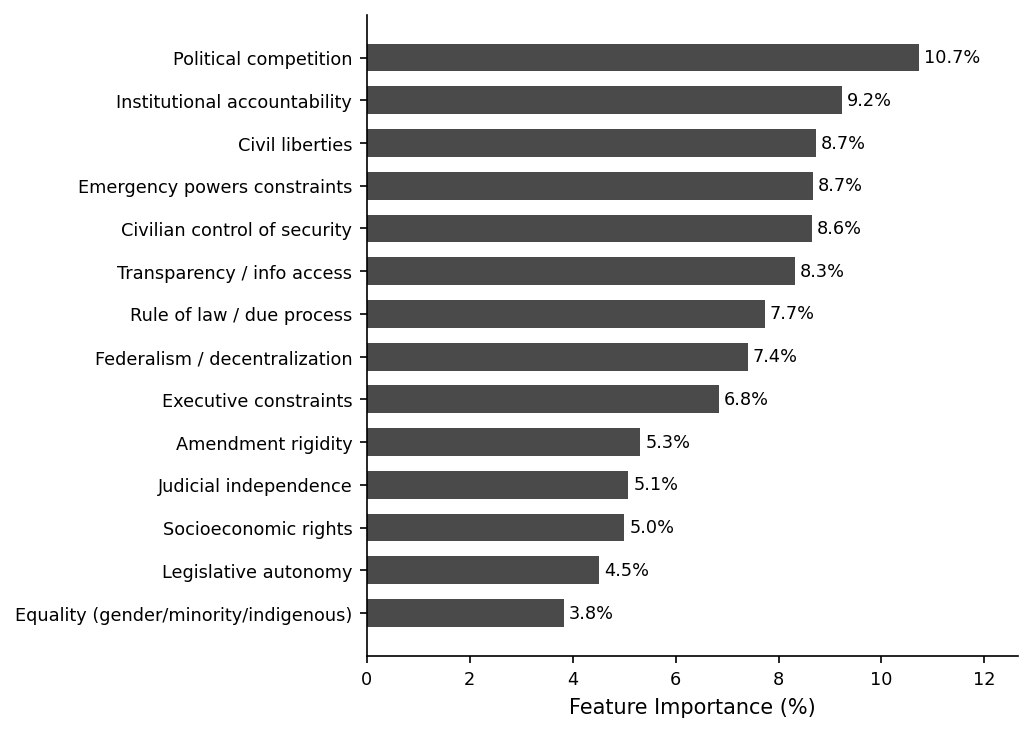
\includegraphics[width=0.75\linewidth]{feature_importances_kfold.png}
\caption{CatBoost feature importances for the Polyarchy prediction model (final model trained on all data). Blue = rights and equality dimensions; green = checks and balances; red = backsliding protections. Classical Madisonian provisions (executive constraints, judicial independence, legislative autonomy) rank in the bottom half.}
\label{fig:feat_imp}
\end{figure}

\subsection*{The Constitutional Gap as a Leading Indicator}

The constitutional gap---the difference between what a country's constitution implies about its democracy and what it actually achieves---is not evenly distributed across countries or time. Countries experiencing democratic backsliding show a characteristic pattern: the gap is near zero or slightly negative in earlier periods (actual democracy meets or slightly exceeds constitutional promise), then widens sharply as actual democratic performance deteriorates while constitutional text remains nominally unchanged. Countries where constitutional provisions function primarily as signals to international audiences rather than as enforceable commitments show a large gap from the outset that never closes. Illustrative cases across both patterns are discussed in the following subsection.

% ---------------------------------------------------------------
\section*{Comparing Constitutional Predictability Across V-Dem's Democracy Concepts}

\subsection*{V-Dem's Five Conceptions of Democracy}

V-Dem does not measure a single concept of democracy but rather five theoretically distinct indices \cite{coppedge_vdem_2024}. \textbf{Electoral Democracy} (Polyarchy, \texttt{v2x\_polyarchy}) requires only that elections be free and fair and that public officials be chosen through them---a minimal procedural standard. \textbf{Liberal Democracy} (\texttt{v2x\_libdem}) adds individual rights protections, an independent judiciary, and constraints on executive power that actually function. \textbf{Egalitarian Democracy} (\texttt{v2x\_egaldem}) further requires that rights and political power be equally distributed across social groups. \textbf{Participatory Democracy} (\texttt{v2x\_partipdem}) emphasizes active citizen participation beyond voting. \textbf{Deliberative Democracy} (\texttt{v2x\_delibdem}) captures the quality of public reasoning in political decisions.

These five conceptions make sharply different demands on constitutional text. Electoral democracy can in principle be tracked purely from constitutional provisions: does the constitution require competitive elections? Does it guarantee universal suffrage? Liberal democracy, by contrast, requires that independent courts actually enforce rights and that executives actually face constraints---outcomes that depend heavily on political culture, state capacity, and enforcement norms not captured in constitutional text.

\subsection*{Results Across Targets}

We re-run the identical CatBoost pipeline---same 14 features, same country-blocked five-fold CV---replacing only the outcome variable. Table~\ref{tab:robustness} reports the results.

\begin{table}[t!]
\centering
\caption{Constitutional predictability across five V-Dem democracy targets.}
\label{tab:robustness}
\begin{tabular}{llcc}
\textbf{Target} & \textbf{V-Dem Index} & \textbf{Fold-avg } $R^2$ & \textbf{RMSE} \\
\midrule
Electoral Democracy     & \texttt{v2x\_polyarchy}  & $0.101 \pm 0.090$ & $0.251$ \\
Egalitarian Democracy   & \texttt{v2x\_egaldem}    & $0.096 \pm 0.086$ & $0.227$ \\
Deliberative Democracy  & \texttt{v2x\_delibdem}   & $0.083 \pm 0.050$ & $0.247$ \\
Participatory Democracy & \texttt{v2x\_partipdem}  & $0.063 \pm 0.080$ & $0.193$ \\
Liberal Democracy       & \texttt{v2x\_libdem}     & $0.052 \pm 0.073$ & $0.243$ \\
\bottomrule
\end{tabular}
\addtabletext{Targets sorted by fold-average $R^2$, highest to lowest. All models use identical 14 constitutional dimension features and country-blocked 5-fold CV.}
\end{table}

\subsection*{Electoral vs.\ Liberal Democracy: The Core Contrast}

The gap between Electoral Democracy ($R^2 = 0.101$) and Liberal Democracy ($R^2 = 0.052$) is the paper's most theoretically informative comparative result. Constitutional text is nearly twice as predictive of electoral democratic outcomes as of liberal democratic ones.

Electoral democracy is a procedural standard: it requires that a constitution mandate competitive elections, guarantee universal suffrage, and protect minimal political freedoms. These provisions are legible in constitutional text---our model can read them directly from the 14 dimension scores. Liberal democracy is harder. It requires that courts actually enforce rights, that executives actually face constraints, that civil liberties are enforceable in practice. These outcomes depend on political culture and state capacity that are simply not captured by what a constitution says. A country can write exactly the right judicial independence provisions while its courts remain politically dependent; it can guarantee civil liberties on paper while its security forces operate with impunity.

The Egyptian constitution's provisions for judicial independence and executive constraints, drafted after 2011, were modeled on liberal democratic templates. They failed not because the provisions were poorly worded but because the de facto balance of power---the military's institutional position, the absence of an independent bar, the lack of civil society capable of enforcing rights---was incompatible with those provisions. Our model, reading only text, would predict a reasonably high liberal democracy score from that constitution; the actual V-Dem score told a different story.

Figure~\ref{fig:feat_imp_comparison} compares feature importances across the two models. The ranking is broadly stable, but two shifts stand out. Transparency / Information Access rises from sixth under Polyarchy to first under Liberal Democracy---consistent with the idea that functioning liberal democracies require informed publics and accountable institutions, not just competitive elections. Political Competition, the top Polyarchy predictor, drops to sixth. Most telling is what does \emph{not} move: Judicial Independence remains eleventh in both rankings, and Legislative Autonomy thirteenth. Even when the outcome explicitly rewards functioning courts and enforced rights, the judicial independence and legislative autonomy provisions written into constitutional text still carry almost no predictive power. The separation-of-powers architecture is no more legible to the model under the liberal democratic standard than under the electoral one.

\begin{figure}[t!]
\centering
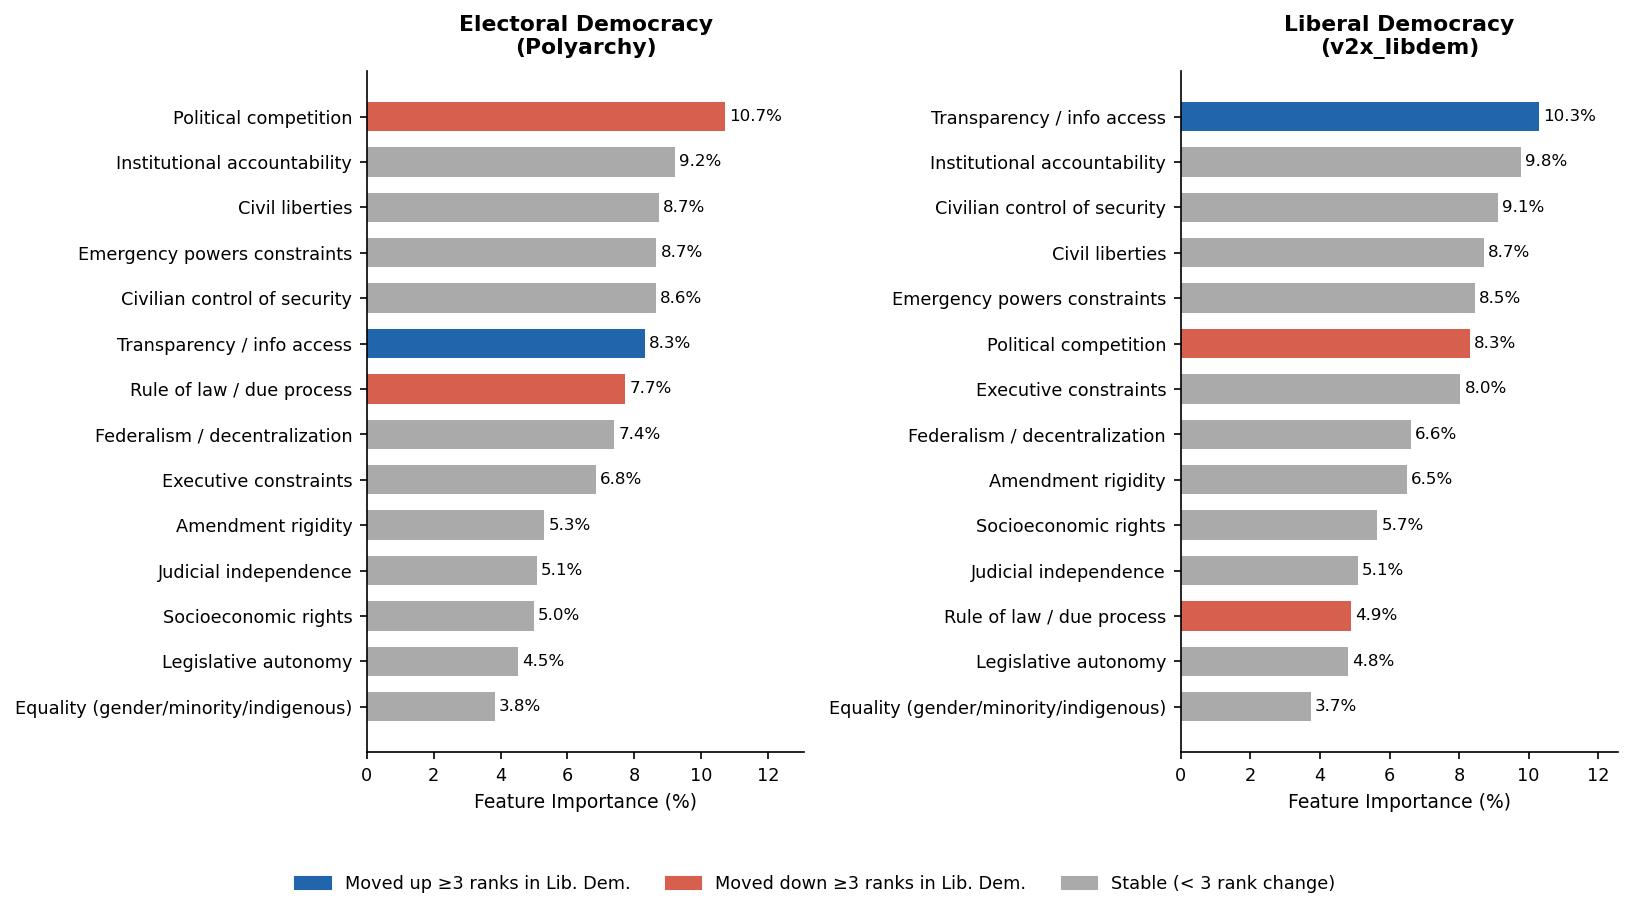
\includegraphics[width=0.75\linewidth]{feature_importances_comparison.png}
\caption{Feature importance rankings for Electoral Democracy (Polyarchy, left) and Liberal Democracy (right). Judicial Independence and Legislative Autonomy rank near the bottom under both targets, while Transparency / Information Access rises to first place under Liberal Democracy.}
\label{fig:feat_imp_comparison}
\end{figure}

\subsection*{Illustrative Cases: Overperformance, Underperformance, and Backsliding}

\textbf{Overperformers} (actual democracy far exceeds constitutional promise): Denmark, New Zealand, Canada, Belgium, and France are the largest positive outliers. These are established democracies whose institutional cultures have built democratic practice well beyond what their formal provisions predict---many operating under constitutional frameworks that are sparse by modern standards, yet sustaining high V-Dem scores through dense networks of norms, judicial conventions, and civil society expectations.

\textbf{Underperformers} (text promises more than the country delivers): Nicaragua, Cuba, Afghanistan, Belarus, and Eritrea show the largest positive gaps---constitutions encoding democratic commitments that ruling regimes have no intention of honoring. The gap for Nicaragua in 2023 is $+0.44$ Polyarchy points; for Cuba, $+0.41$. These are cases where constitutional text functions primarily as window-dressing for international audiences.

\textbf{Backsliding cases} (gap widens as democracy deteriorates while text stays intact): Hungary (post-2010 Orb\'an consolidation), Venezuela (post-Ch\'avez erosion), and Turkey (post-2016 constitutional referendum) show a characteristic temporal pattern. In earlier periods the gap is near zero; it then widens sharply as actual democratic performance deteriorates while constitutional text remains nominally unchanged---consistent with Levitsky and Ziblatt's \cite{levitsky_ziblatt_2018} account of democratic erosion from within.

\textbf{Constitutional engineering failures} (gap large from the outset): Egypt (post-2011 Arab Spring) and Lebanon (1989 Taif Agreement) illustrate the limits of constitutional design from a different angle. In both cases, well-drafted provisions were adopted in the wake of political crises, but the de facto conditions needed to enforce them---an independent judiciary, functioning civil society, settled elite bargains---were absent from the start. The gap between constitutional promise and democratic reality was large from day one and never closed.

% ---------------------------------------------------------------
\section*{Constitutional Age, Norms, and the Gap}

\subsection*{The Older the Constitution, the Stronger the Democracy}

One of the more striking patterns in the data concerns not what a constitution says but how long it has been in place. Countries with older constitutions consistently outperform what their text would predict, while newly adopted constitutions tend to fall short of it. This gap inverts around 30 years of age: new constitutions are associated with democratic under-delivery; older ones are embedded in countries that have outgrown their text entirely.

The historical picture in Figure~\ref{fig:inflation} makes this concrete. Constitutions adopted before World War I are spare documents that do not enumerate the extensive rights modern drafters consider standard, yet the countries still operating under them are among the world's strongest democracies. The opposite is true of post-Cold War constitutions: rich in democratic provisions, often drafted with international advisers, yet the countries that adopted them frequently fall short of the democratic levels they promise. Each successive wave of constitution-writing has produced documents with higher ambitions, but ambition has not translated into performance at the same rate: the older the constitution, the more likely a country is to have outgrown its text.

\begin{figure}[t!]
\centering

\includegraphics[width=0.75\linewidth]{constitution_inflation.png}
\caption{Constitutional promise and actual democracy by adoption era. The older the constitution, the more actual democracy exceeds what the text implies. Recent constitutions promise more but deliver less relative to their provisions.}
\label{fig:inflation}
\end{figure}

\subsection*{Norms Take Time}

The most natural interpretation of these patterns is that what makes constitutions effective is not the text but what grows up around it over time. Countries like the United Kingdom, Denmark, and New Zealand have operated under their constitutional frameworks long enough that dense networks of institutional norms have formed---judicial conventions, legislative customs, civil society expectations---that enforce democratic behavior whether or not the written document requires it. The constitution is no longer just a legal document; it is a focal point for political culture.

New constitutions have not yet had time to develop that culture. Egypt's 2014 constitution, Lebanon's Taif amendments, and Myanmar's 2008 document all score reasonably well on our 14 constitutional dimensions. Their actual democratic performance reflects not inadequate drafting but the absence of the institutional ecology that gives constitutional text its force. Writing the right provisions is a necessary starting point, but it is not sufficient---and the data suggest that the gap between text and reality is at its widest precisely when countries need their constitutions most: in the early years of a transition, when democratic norms are fragile and enforcement is weakest.

% ---------------------------------------------------------------
\section*{How Constitutional Provisions Have Evolved}

The 14 dimension scores also reveal what constitution-writers have actually prioritized across history. Figure~\ref{fig:dim_change} plots the absolute change in each dimension's global average score from the 1900s to the 2020s, computed across all country-years in the dataset.

\begin{figure}[t!]
\centering

\includegraphics[width=0.75\linewidth]{dimension_change_bar.png}
\caption{Absolute change in global average constitutional dimension scores from the 1900s to the 2020s. Socioeconomic Rights, Equality, and Civil Liberties have grown most; the classical separation-of-powers dimensions have barely moved.}
\label{fig:dim_change}
\end{figure}

The pattern reinforces the paper's central argument from an unexpected angle. The dimensions that have grown most over the past century are Socioeconomic Rights ($+0.31$), Equality ($+0.20$), Civil Liberties ($+0.17$), and Rule of Law / Due Process ($+0.17$)---the modern rights-expansion provisions that characterize successive waves of post-war and post-colonial constitution-writing. By contrast, the classical Madisonian architecture---Executive Constraints ($+0.02$), Legislative Autonomy ($+0.004$), Emergency Powers Constraints ($\approx 0$)---has been essentially flat. These provisions were already present in early constitutions and have not meaningfully deepened.

This helps explain the feature importance results. The separation-of-powers dimensions rank low as predictors not because they are unimportant for democracy, but because they vary so little across constitutions: nearly every country has written them in. What discriminates democratic from undemocratic countries today is not whether a constitution has executive constraints on paper, but whether it has built the rights and competition provisions that are harder to adopt insincerely.

% ---------------------------------------------------------------
\section*{Democratic Culture and Institutional Ecology}

\textbf{Interpretive caveat.} The results in this section should be read as descriptive rather than causal. Democratic culture and democratic performance are mutually reinforcing: countries that sustain democratic institutions develop the civic norms that make those institutions resilient, and those norms in turn enable further consolidation. A country's EIU culture score is partly a record of how democracy has already played out within it. We therefore treat culture as a structured correlate of the residual variance left unexplained by constitutional text, not as an independent causal lever.

The age finding raises a natural question: is age itself the mechanism, or a proxy for something that accumulates over time? The most direct candidate is democratic culture. We test this using the EIU Democratic Culture Index \cite{eiu_democracy_index}, a survey-based measure scored 0--10. Adding this single variable to the CatBoost model raises the out-of-fold $R^2$ from $0.07$ to $0.40$ on the subset of country-years with EIU coverage (2006--2023). An interaction specification reveals that the marginal effect of constitutional text varies sharply across culture levels: at low culture scores (EIU~$\approx 4$), a one-unit increase in constitutional score shifts predicted democracy by $0.63$ points; at high culture scores (EIU~$\approx 8$), that marginal effect collapses to $0.08$. Constitutions appear nearly inert in low-culture environments regardless of how well they are written; in high-culture environments, democratic performance has already outgrown the text. These results confirm that the residual left unexplained by constitutional provisions is structured and not random---consistent with the age-based evidence---but cannot be read as a causal finding. The relationship between democratic culture, constitutional design, and institutional consolidation is an area the author is actively exploring in ongoing work.

% ---------------------------------------------------------------
\section*{Limitations}

The primary methodological limitation concerns the LLM-assisted coding. The weights and value maps assigned by the language model reflect the model's implicit theory of constitutional design, and different prompting strategies or model versions could in principle produce different results. To mitigate this, we explored several alternative approaches before settling on the current typology. These included feeding raw constitutional texts directly to the LLM for scoring, and constructing multiple alternative typologies with different variable groupings and dimension definitions. Upon systematic manual review against the CCPCNC codings and known constitutional contexts, the current CCPCNC-based typology---in which the LLM assigns weights and value maps to pre-structured variable codings rather than interpreting raw text---produced the most consistent and interpretable results. The manual audit of 10 constitutions across different time periods and regime types, described in the Data and Measurement section, provides additional confidence. Nonetheless, a full inter-rater reliability assessment with independent human coders assigning weights to the same variables would provide stronger validation and is an important direction for future work.

% ---------------------------------------------------------------
\section*{Conclusion}

Constitutional text contains real but limited information about democratic performance. In out-of-country prediction, the provisions most associated with democracy are not the classical Madisonian safeguards of separated powers, judicial independence, and legislative autonomy, but provisions structuring political competition, institutional accountability, and civil liberties. The gap between constitutional promise and democratic reality is largest in newer constitutions and in regimes where democratic norms and enforcement capacity have not consolidated.

This paper tested these claims systematically across 17,390 country-year observations spanning 1789--2023. A gradient-boosted model trained on 14 constitutional dimension scores achieves an out-of-fold $R^2$ of roughly 0.10 on entirely unseen countries---well above chance but far from deterministic. The provisions that best predict democracy are those governing Political Competition, Institutional Accountability, and Civil Liberties, not the classical separation-of-powers architecture, which clusters near the bottom of the feature importance distribution regardless of whether the target is electoral or liberal democracy.

The constitutional gap is not random noise. It is structured by constitutional age: documents that have survived for decades are embedded in countries that have consistently outperformed their text, while newly adopted constitutions, however rights-laden, are systematically associated with democratic under-delivery. The most parsimonious interpretation is that what makes constitutional provisions effective over time is not the text itself but the institutional ecology---norms, expectations, enforcement capacity---that accumulates around them. Democratic culture, when measured directly, confirms this, though because democracy and culture develop together rather than independently, that explanatory power cannot be cleanly attributed to culture as a separable cause.

Taken together, the findings counsel skepticism about constitutional engineering as a reliable path to democracy. The provisions that post-transition governments most reliably import---judicial independence clauses, executive constraint mechanisms, bicameral checks---are exactly the ones that carry the least predictive signal in the data. This does not mean such provisions are unimportant; it means that writing them into a document is not, by itself, what makes them effective. What makes them effective is the de facto political environment that gives them teeth---the very thing that constitutional text, standing alone, cannot supply.

% ---------------------------------------------------------------

\acknow{The author thanks the instructors and teaching assistants of QSS 45 for guidance throughout this project. Computational resources were provided by Dartmouth Research Computing. Data from the Comparative Constitutions Project and V-Dem Institute were used under their respective open-access licenses.}

\showacknow

\bibliography{references}

\end{document}
